\documentclass[ignorenonframetext,]{beamer}
\setbeamertemplate{caption}[numbered]
\setbeamertemplate{caption label separator}{: }
\setbeamercolor{caption name}{fg=normal text.fg}
\beamertemplatenavigationsymbolsempty
\usepackage{lmodern}
\usepackage{amssymb,amsmath}
\usepackage{ifxetex,ifluatex}
\usepackage{fixltx2e} % provides \textsubscript
\ifnum 0\ifxetex 1\fi\ifluatex 1\fi=0 % if pdftex
  \usepackage[T1]{fontenc}
  \usepackage[utf8]{inputenc}
\else % if luatex or xelatex
  \ifxetex
    \usepackage{mathspec}
  \else
    \usepackage{fontspec}
  \fi
  \defaultfontfeatures{Ligatures=TeX,Scale=MatchLowercase}
\fi
\usetheme[]{boxes}
\usecolortheme{structure}
% use upquote if available, for straight quotes in verbatim environments
\IfFileExists{upquote.sty}{\usepackage{upquote}}{}
% use microtype if available
\IfFileExists{microtype.sty}{%
\usepackage{microtype}
\UseMicrotypeSet[protrusion]{basicmath} % disable protrusion for tt fonts
}{}
\newif\ifbibliography
\hypersetup{
            pdftitle={miniBeamer RMD\_TO\_PDF initial presentation},
            pdfauthor={mckraqs},
            pdfborder={0 0 0},
            breaklinks=true}
\urlstyle{same}  % don't use monospace font for urls
\usepackage{color}
\usepackage{fancyvrb}
\newcommand{\VerbBar}{|}
\newcommand{\VERB}{\Verb[commandchars=\\\{\}]}
\DefineVerbatimEnvironment{Highlighting}{Verbatim}{commandchars=\\\{\}}
% Add ',fontsize=\small' for more characters per line
\newenvironment{Shaded}{}{}
\newcommand{\KeywordTok}[1]{\textcolor[rgb]{0.00,0.00,1.00}{#1}}
\newcommand{\DataTypeTok}[1]{#1}
\newcommand{\DecValTok}[1]{#1}
\newcommand{\BaseNTok}[1]{#1}
\newcommand{\FloatTok}[1]{#1}
\newcommand{\ConstantTok}[1]{#1}
\newcommand{\CharTok}[1]{\textcolor[rgb]{0.00,0.50,0.50}{#1}}
\newcommand{\SpecialCharTok}[1]{\textcolor[rgb]{0.00,0.50,0.50}{#1}}
\newcommand{\StringTok}[1]{\textcolor[rgb]{0.00,0.50,0.50}{#1}}
\newcommand{\VerbatimStringTok}[1]{\textcolor[rgb]{0.00,0.50,0.50}{#1}}
\newcommand{\SpecialStringTok}[1]{\textcolor[rgb]{0.00,0.50,0.50}{#1}}
\newcommand{\ImportTok}[1]{#1}
\newcommand{\CommentTok}[1]{\textcolor[rgb]{0.00,0.50,0.00}{#1}}
\newcommand{\DocumentationTok}[1]{\textcolor[rgb]{0.00,0.50,0.00}{#1}}
\newcommand{\AnnotationTok}[1]{\textcolor[rgb]{0.00,0.50,0.00}{#1}}
\newcommand{\CommentVarTok}[1]{\textcolor[rgb]{0.00,0.50,0.00}{#1}}
\newcommand{\OtherTok}[1]{\textcolor[rgb]{1.00,0.25,0.00}{#1}}
\newcommand{\FunctionTok}[1]{#1}
\newcommand{\VariableTok}[1]{#1}
\newcommand{\ControlFlowTok}[1]{\textcolor[rgb]{0.00,0.00,1.00}{#1}}
\newcommand{\OperatorTok}[1]{#1}
\newcommand{\BuiltInTok}[1]{#1}
\newcommand{\ExtensionTok}[1]{#1}
\newcommand{\PreprocessorTok}[1]{\textcolor[rgb]{1.00,0.25,0.00}{#1}}
\newcommand{\AttributeTok}[1]{#1}
\newcommand{\RegionMarkerTok}[1]{#1}
\newcommand{\InformationTok}[1]{\textcolor[rgb]{0.00,0.50,0.00}{#1}}
\newcommand{\WarningTok}[1]{\textcolor[rgb]{0.00,0.50,0.00}{\textbf{#1}}}
\newcommand{\AlertTok}[1]{\textcolor[rgb]{1.00,0.00,0.00}{#1}}
\newcommand{\ErrorTok}[1]{\textcolor[rgb]{1.00,0.00,0.00}{\textbf{#1}}}
\newcommand{\NormalTok}[1]{#1}
\usepackage{longtable,booktabs}
\usepackage{caption}
% These lines are needed to make table captions work with longtable:
\makeatletter
\def\fnum@table{\tablename~\thetable}
\makeatother
\usepackage{graphicx,grffile}
\makeatletter
\def\maxwidth{\ifdim\Gin@nat@width>\linewidth\linewidth\else\Gin@nat@width\fi}
\def\maxheight{\ifdim\Gin@nat@height>\textheight0.8\textheight\else\Gin@nat@height\fi}
\makeatother
% Scale images if necessary, so that they will not overflow the page
% margins by default, and it is still possible to overwrite the defaults
% using explicit options in \includegraphics[width, height, ...]{}
\setkeys{Gin}{width=\maxwidth,height=\maxheight,keepaspectratio}

% Prevent slide breaks in the middle of a paragraph:
\widowpenalties 1 10000
\raggedbottom

\AtBeginPart{
  \let\insertpartnumber\relax
  \let\partname\relax
  \frame{\partpage}
}
\AtBeginSection{
  \ifbibliography
  \else
    \let\insertsectionnumber\relax
    \let\sectionname\relax
    \frame{\sectionpage}
  \fi
}
\AtBeginSubsection{
  \let\insertsubsectionnumber\relax
  \let\subsectionname\relax
  \frame{\subsectionpage}
}

\setlength{\parindent}{0pt}
\setlength{\parskip}{6pt plus 2pt minus 1pt}
\setlength{\emergencystretch}{3em}  % prevent overfull lines
\providecommand{\tightlist}{%
  \setlength{\itemsep}{0pt}\setlength{\parskip}{0pt}}
\setcounter{secnumdepth}{0}
% \setmainfont{Roboto Condensed}
% \setsansfont[BoldFont=Roboto Bold]{Roboto Condensed}
% \setmonofont[Scale=MatchLowercase]{Inconsolata}

\usepackage[export]{adjustbox}
\usepackage{xcolor}
\usepackage{tikz}

% Fonts only work with xelatex
% \usepackage{fontspec}

% \defaultfontfeatures{Mapping=tex-text}
% \usefonttheme{serif}
% \setmainfont{Adagio_Slab-Regular.otf}
% \setbeamerfont{title}{family=\fontspec{RadikalWUT-Bold.otf}}
% \setbeamerfont{title page}{family=\fontspec{RadikalWUT-Bold.otf}}
% \setbeamerfont{frametitle}{family=\fontspec{RadikalWUT-Bold.otf}}
% \setbeamerfont{frame title}{family=\fontspec{RadikalWUT-Bold.otf}}

\logo{\vspace*{-2mm}\makebox[\paperwidth]{\hspace*{2mm}{}\hfill{}}}
\AtBeginPart{}
\AtBeginSection{}
\AtBeginSubsection{}
\AtBeginSubsubsection{}
\setlength{\emergencystretch}{0em}
\setlength{\parskip}{0pt}

\setbeamerfont{myTOC}{series=\bfseries,size=\large}
\AtBeginSection[]{\frame{\frametitle{Outline}%
                  \usebeamerfont{myTOC}\tableofcontents[current]}}

\definecolor{SAPPHIRE}{RGB}{120, 150, 207}
\definecolor{MOKKA}{RGB}{100, 90, 90}
\definecolor{GRAPHITE}{RGB}{60, 60, 76}
\definecolor{HEATHER}{RGB}{180, 160, 170}
\definecolor{BLACK}{RGB}{0, 0, 0}
\definecolor{WHITE}{RGB}{255, 255, 255}
\definecolor{blue}{rgb}{.0,.15,.55}

% \usepackage{fontawesome}
\setbeamertemplate{frametitle}{\vspace{.75em}\color{GRAPHITE}\bfseries\insertframetitle}
\setbeamertemplate{navigation symbols}{}

\setbeamertemplate{itemize item}{\color{GRAPHITE}\scriptsize{$\bullet$}}
\setbeamertemplate{itemize subitem}{\color{GRAPHITE}\tiny{$\bullet$}}
% \setbeamertemplate{background}{\tikz[overlay,remember picture]\node[opacity=0.05]at (current page.center){\includegraphics[width=10cm]{BACKGROUND}};}

\setbeamerfont{title}{series=\bfseries,parent=structure,size=\LARGE}
\setbeamerfont{subtitle}{series=\bfseries,parent=structure,size=\Large}
\setbeamerfont{titlelike}{series=\bfseries,size=\Huge}

\usepackage{color,hyperref}
\hypersetup{colorlinks,breaklinks,
  linkcolor=GRAPHITE,urlcolor=blue,citecolor=blue}
\usepackage{url}
\urlstyle{same}

\setbeamercolor{title}{fg=GRAPHITE}
\setbeamercolor{subtitle}{fg=GRAPHITE}
\setbeamercolor{normal text}{fg=GRAPHITE}
\setbeamercolor{normal text}{bg=SAPPHIRE}
\setbeamercolor{titlelike}{fg=GRAPHITE}
\setbeamercolor{structure}{fg=GRAPHITE}
\setbeamercolor{section in toc}{parent=GRAPHITE}

\title{miniBeamer RMD\_TO\_PDF initial presentation}
\author{mckraqs}
\date{}

\begin{document}
\frame{\titlepage}

% ***
% beforebody.tex template, feel free to use it
% ***

\section[]{}
\frame{\small \frametitle{Table of Contents} \tableofcontents}

\begin{frame}{miniBeamer PDF presentation with R Markdown}

Get it from GitHub: \url{https://github.com/mckraqs/miniBeamer}

\end{frame}

\section{R Markdown}\label{r-markdown}

\begin{frame}{R Markdown}

This is an R Markdown presentation. Markdown is a simple formatting
syntax for authoring HTML, PDF, and MS Word documents. For more details
on using R Markdown see \url{http://rmarkdown.rstudio.com}.

When you click the \textbf{Knit} button a document will be generated
that includes both content as well as the output of any embedded R code
chunks within the document.

\end{frame}

\section{Shower introduction}\label{shower-introduction}

\begin{frame}{Shower introduction}

These slides use a template from the
\href{https://github.com/shower/shower}{shower} presentation system.
Notable features:

\begin{enumerate}
\def\labelenumi{\arabic{enumi}.}
\tightlist
\item
  Works in all modern browsers
\item
  Presentation fully keyboard accessible
\item
  Multiple themes available
\item
  Printable to PDF
\end{enumerate}

Shower noun. A person or thing that shows.

\end{frame}

\begin{frame}{Lists}

\begin{enumerate}
\def\labelenumi{\arabic{enumi}.}
\tightlist
\item
  Simple lists are marked with bullets
\item
  Ordered lists begin with a number
\item
  You can even nest lists one inside another

  \begin{itemize}
  \tightlist
  \item
    Or mix their types
  \item
    But do not go too far
  \item
    Otherwise audience will be bored
  \end{itemize}
\item
  Look, seven rows exactly!
\end{enumerate}

\end{frame}

\begin{frame}{Formulas}

Formulas are rendered by KaTeX, \url{https://github.com/Khan/KaTeX}

It supports both inline: \(y = x / 2\) and displayed formulas:

\[ x_{1,2} = \frac{- b \pm \sqrt{b^2 - 4ac}}{2a} \]

\end{frame}

\begin{frame}{Slide with quote}

\begin{quote}
Learning more about programming is a long-term investment: it won't pay
off immediately, but in the long term it will allow you to solve new
problems more quickly, and let you reuse your insights from previous
problems in new scenarios.
\end{quote}

\textbf{Hadley Wickham}

\end{frame}

\begin{frame}[fragile]{Slide with R Code and Output}

\begin{itemize}
\tightlist
\item
  Some text \scriptsize
\end{itemize}

\begin{Shaded}
\begin{Highlighting}[]
\NormalTok{hw <-}\StringTok{ }\DecValTok{2} \OperatorTok{+}\StringTok{ }\DecValTok{2}
\NormalTok{hw}
\NormalTok{## [1] 4}
\end{Highlighting}
\end{Shaded}

\end{frame}

\begin{frame}{Tables}

\begin{longtable}[]{@{}ccccc@{}}
\toprule
& mpg & cyl & disp & hp\tabularnewline
\midrule
\endhead
Mazda RX4 & 21 & 6 & 160 & 110\tabularnewline
Mazda RX4 Wag & 21 & 6 & 160 & 110\tabularnewline
Datsun 710 & 22.8 & 4 & 108 & 93\tabularnewline
Hornet 4 Drive & 21.4 & 6 & 258 & 110\tabularnewline
Hornet Sportabout & 18.7 & 8 & 360.0 & 175\tabularnewline
Valiant & 18.1 & 6 & 225.0 & 105\tabularnewline
Duster 360 & 14.3 & 8 & 360.0 & 245\tabularnewline
\bottomrule
\end{longtable}

\end{frame}

\begin{frame}{Lists item by item}

\begin{enumerate}[<+->]
\def\labelenumi{\arabic{enumi}.}
\tightlist
\item
  Lets you reveal list items one by one
\item
  To keep some key points
\item
  In secret from audience
\item
  But it will work only once
\item
  Nobody wants to see the same joke twice
\end{enumerate}

\end{frame}

\section{Cat image!}\label{cat-image}

\begin{frame}{Cat image!}

\begin{figure}
\centering
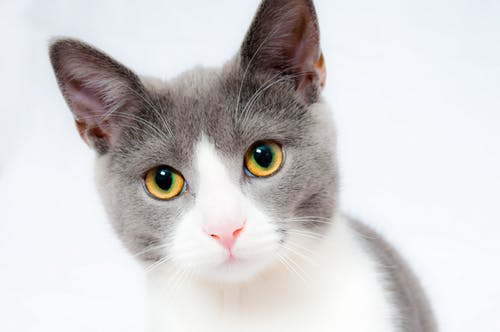
\includegraphics{cat.jpeg}
\caption{Pretty cat}
\end{figure}

\end{frame}

\begin{frame}{Slide with Plot}

\scriptsize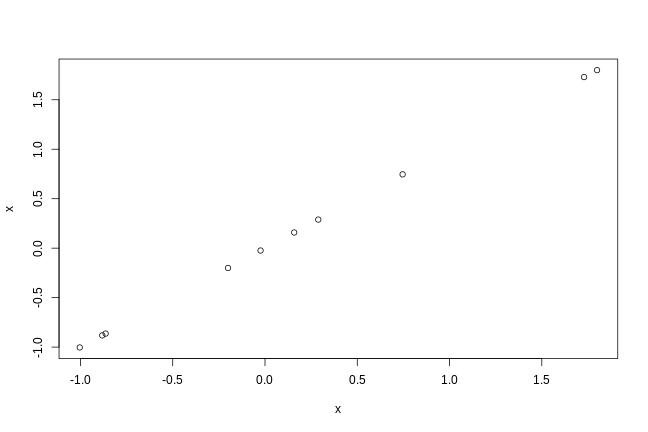
\includegraphics{rmd_to_beamer_example_files/figure-beamer/unnamed-chunk-3-1.jpeg}

\end{frame}

% ***
% afterbody.tex template, feel free to use it
% File generated thanks to mckraqs/miniBeamer package!
% ***

\end{document}
